
\begin{frame}{Locomotion Problem}

\begin{columns}

\column{0.5\linewidth}

\scalebox{0.65}{
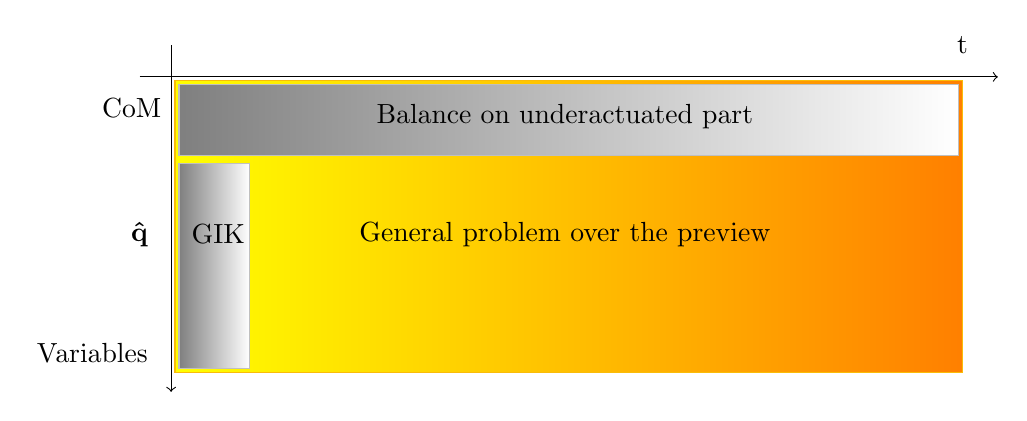
\begin{tikzpicture}
  \draw [->] (-0.4,0) -- (10.5,0);
  \draw [->] (0,0.4) -- (0,-4);
  \shadedraw[left color=yellow, right color= orange, draw=yellow!50!orange](0.05,-0.05) rectangle (10.05,-3.75);
  \shadedraw[left color=gray, right color= white, draw=gray!50!white] (0.1,-0.1) rectangle (10,-1.0);
  \shadedraw[left color=gray, right color= white, draw=gray!50!white](0.1,-1.1) rectangle (1,-3.7);
  \draw (10.05,0.4) node {t};
  \draw (-0.5,-0.4) node {CoM};
  \draw (-0.4,-2.0) node {${\bf \hat{q} }$};
  \draw (-1.0,-3.5) node {Variables};
  \draw (5,-0.5) node {Balance on underactuated part};
  \draw (0.6,-2.0) node {GIK};
  \draw (5,-2.0) node {General problem over the preview};
\end{tikzpicture}
}

\column{0.5\linewidth}
\hspace*{1.2cm}
\scalebox{0.8}{
  \begin{tikzpicture}[remember picture]
	  \node (pic) at (0,0) {\includegraphics[width=0.38\paperwidth]{./images/HRP-2-Nishiwaki-Alone}};
	%  \node (pic) at (2.7,3.6) {\includegraphics[width=0.8\linewidth]{./images/HRP-2-Nishiwaki-Alone}};
	
	%  \draw[help lines] (1,1) grid (5,6);         
	%  \draw (0,0) {(0,0)};         
  \node (lf) at ([shift={(-0.5,-1.63)}]pic) {};
	  \ExtractCoordinate{$(lf)$};
	  \draw[color=darkgreen, left color=green, right color=green!60, 
	    xshift=\XCoord,yshift=\YCoord, drop shadow={ashadow, color=green!60!black}] [rotate=100,scale=0.15] 
	  \arrowt;
	
	  \node (rf) at ([shift={(0.4,-1.44)}]pic) {};
	  \ExtractCoordinate{$(rf)$};
	  \draw[color=darkgreen, left color=green, right color=green!60, 
	    xshift=\XCoord,yshift=\YCoord, drop shadow={ashadow, color=green!60!black}] [rotate=100,scale=0.15] 
	  \arrowt;
	\end{tikzpicture}
}
\end{columns}
\begin{center}
\begin{minipage}{0.31\linewidth}
HRP-2 (36 DoFs)\\
control period (5ms)\\
preview duration (1.6s)
\end{minipage} 
 = 10 000 variables : \textbf{No real time computation}
\end{center}

\end{frame}
%%%%%%%%%%%%%%%%%%%%%%%%%%%%%%%%%%%%%%%%%%%%%%%%%%%%%%%%%%%%%%%%%%%%%%%%%%%%%%%%%%%%%
\begin{frame}{
Dynamics - \only<1> {Whole Body}\only<2> {Mixed}\only<3>{Centroidal}\only<4>{Linearized Inverted Pendulum} Model
}
  \vskip -0.5cm
  \begin{columns}[t]
%%
    \begin{column}[T]{0.5\linewidth}
    \only<1>{
      \begin{alertblock}{No approximation}
        [Koch Humanoids 2014] Step over 20$cm$ high obstacle (hours/days)
      \end{alertblock}
      \vspace*{-0.2cm}
      \begin{alertblock}{Approximation on contact}
        [Todorov ICRA 2014] No walk feasible on the robot (100ms)
        Continuous contact model
      \end{alertblock}
    }
    \only<2>{
      \begin{alertblock}{Mixed Formulation}
        [Kuindersma Autonomous Robots 2015]
        
        [Sherikov PhD Thesis 2016]
      \end{alertblock}
      \vspace*{-0.8cm}
    }
    \only<3>{
      \begin{alertblock}{3D PG - *}
        [Hirukawa ICRA 2007]
        
        $\dot{\bf \am}=0$ ; Contacts and Forces Distribution Known
        
        [Perrin IJRR 2015]
        
        $\dot{\bf \am}=0$ ; Forces Direction Known
      \end{alertblock}
      \vspace*{-0.8cm}
      \begin{align*}
        &m\,( \mathbf{ \ddot{c} } - \mathbf{g}) = \sum_{i} \mathbf{R} _{i} \mathbf{f} _{i}\\
        &\dot{\bf \am} = \sum_{i} (\mathbf{p} _{i}-\mathbf{c}) \times \mathbf{R} _{i} \mathbf{f} _{i} + \mathbf{R} _{i} \mathbf{\tau}_i \\
        & \text{Balance criteria (e.g. Coulomb law)}
      \end{align*}    
    }
    \only<4>{
      \begin{alertblock}{2D PG - *}
        [Herdt Advanced Robotics 2010]        
        [Sherikov Humanoids 2014]
      \end{alertblock}
      \vspace*{-0.3cm}
      \begin{alertblock}{Linearized Inverted Pendulum Model}
        \itemd coplanar contact
      
        \itemd $\dot{\bf \am} = 0$ \itemd $c^z = cst$ \itemd ${\bf p}=CoP$
      \end{alertblock}
      \vspace*{-0.5cm}
      \begin{equation*}
        \left\lbrace
        \begin{aligned}
          p_{x} = c_x - \frac{c_z}{g}\ddot{c}_x \\
          p_{y} = c_y - \frac{c_z}{g}\ddot{c}_y \\
          {\bf p} \in \text{Support Polygon}
        \end{aligned}
        \right.
      \end{equation*}
    }
    \end{column}

    %

    \begin{column}[T]{0.4\linewidth}    
    %\vskip 1cm
	  \scalebox{0.4}{
		\begin{tikzpicture}
		  \draw [->] (-0.4,0) -- (10.5,0);
		  \draw [->] (0,0.4) -- (0,-4);
		  \only<1>{
		  \shadedraw[left color=yellow, right color= orange, draw=yellow!50!orange](0.05,-0.05) rectangle (10.05,-3.75);}
		  \shadedraw[left color=gray, right color= white, draw=gray!50!white] (0.1,-0.1) rectangle (10,-1.0);
		  \shadedraw[left color=gray, right color= white, draw=gray!50!white](0.1,-1.1) rectangle (1,-3.7);
		  \only<2>{
		  \draw [color=blue,line width=4pt,->] (0.5,-1.5) -- node {} (0.5,-0.5);
		  }
		  \only<2->{
		  \draw [color=blue,line width=4pt,->] (0.5,-0.5) -- node {} (0.5,-1.5);
		  }
		  \draw (10.05,0.4) node {t};
		  \draw (-0.5,-0.4) node {CoM};
		  \draw (-0.4,-2.0) node {${\bf \hat{q} }$};
		  \draw (-1.0,-3.5) node {Variables};
		  \draw (5,-0.5) node {Balance on underactuated part};
		  \draw (0.6,-2.0) node {GIK};
		  \only<1>{\draw (5,-2.0) node {General problem over the preview};}
		\end{tikzpicture}
	  }
	  \vspace*{-0.2cm}
    \only<1>{
      \scalebox{0.8}{
         \begin{tikzpicture}[remember picture]
				  \node (pic) at (0,0) {\includegraphics[width=0.38\paperwidth]{./images/HRP-2-Nishiwaki-Alone}};
			  \node (lf) at ([shift={(-0.5,-1.63)}]pic) {};
				  \ExtractCoordinate{$(lf)$};
				  \draw[color=darkgreen, left color=green, right color=green!60, 
				    xshift=\XCoord,yshift=\YCoord, drop shadow={ashadow, color=green!60!black}] [rotate=100,scale=0.15] 
				  \arrowt;
				
				  \node (rf) at ([shift={(0.4,-1.44)}]pic) {};
				  \ExtractCoordinate{$(rf)$};
				  \draw[color=darkgreen, left color=green, right color=green!60, 
				    xshift=\XCoord,yshift=\YCoord, drop shadow={ashadow, color=green!60!black}] [rotate=100,scale=0.15] 
				  \arrowt;
				\end{tikzpicture}
       }
     }
     \only<2-3>{
       \scalebox{0.8}{\begin{tikzpicture}[remember picture]
  \node (pic) at (0,0) {\includegraphics[width=0.38\paperwidth]{./images/HRP-2-Nishiwaki-Alone}};
%  \node (pic) at (2.7,3.6) {\includegraphics[width=0.8\linewidth]{./images/HRP-2-Nishiwaki-Alone}};

%  \draw[help lines] (1,1) grid (5,6);         
%  \draw (0,0) {(0,0)};         
  \node (com) at ([shift={(-0.2,0.8)}]pic) {};
  \draw[color=black,fill=white,line width=0.3mm,rotate around={40:(2.3,4.1)}] ([shift={(-0.2,0.2)}]com) ellipse (0.6cm and 0.4cm);
  \draw[color=black,fill=white,line width=0.3mm] (com) arc (0:360:0.3cm);
  \draw[fill=black] ([shift={(-0.3,0.3)}]com) arc (90:180:0.3cm) -- +(0.3cm,0cm) -- +(0.6cm,0cm) arc(360:270:0.3cm);
  
  \node (purparr) at ([shift={(-0.15,-0.1)}]com) {};
  \ExtractCoordinate{$(purparr)$};
  \draw[color=violet, left color=magenta, right color=magenta!60, 
    xshift=\XCoord,yshift=\YCoord, drop shadow={ashadow, color=magenta!60!black}] [rotate=180]
  \arrowtd;

  \node (lf) at ([shift={(-0.5,-1.63)}]pic) {};
  \ExtractCoordinate{$(lf)$};
  \draw[color=darkgreen, left color=green, right color=green!60, 
    xshift=\XCoord,yshift=\YCoord, drop shadow={ashadow, color=green!60!black}] [rotate=100,scale=0.15] 
  \arrowt;

  \node (rf) at ([shift={(0.4,-1.44)}]pic) {};
  \ExtractCoordinate{$(rf)$};
  \draw[color=darkgreen, left color=green, right color=green!60, 
    xshift=\XCoord,yshift=\YCoord, drop shadow={ashadow, color=green!60!black}] [rotate=100,scale=0.15] 
  \arrowt;
\end{tikzpicture}}
     }
     \only<4>{
       \scalebox{0.7}{\begin{tikzpicture}[remember picture]
  \node (pic) at (0,0) {\includegraphics[width=0.38\paperwidth]{./images/HRP-2-Nishiwaki-Alone}};
%  \node (pic) at (2.7,3.6) {\includegraphics[width=0.8\linewidth]{./images/HRP-2-Nishiwaki-Alone}};

%  \draw[help lines] (1,1) grid (5,6);         
%  \draw (0,0) {(0,0)};         
  \node (com) at ([shift={(-0.2,0.8)}]pic) {};
  \draw[color=black,fill=white,line width=0.3mm,rotate around={40:(2.3,4.1)}] ([shift={(-0.2,0.2)}]com) ellipse (0.6cm and 0.4cm);
  \draw[color=black,fill=white,line width=0.3mm] (com) arc (0:360:0.3cm);
  \draw[fill=black] ([shift={(-0.3,0.3)}]com) arc (90:180:0.3cm) -- +(0.3cm,0cm) -- +(0.6cm,0cm) arc(360:270:0.3cm);
  
  \node (purparr) at ([shift={(-0.15,-0.1)}]com) {};
  \ExtractCoordinate{$(purparr)$};
  \draw[color=violet, left color=magenta, right color=magenta!60, 
    xshift=\XCoord,yshift=\YCoord, drop shadow={ashadow, color=magenta!60!black}] [rotate=180]
  \arrowtd;

  \node (lf) at ([shift={(-0.5,-1.63)}]pic) {};
  \ExtractCoordinate{$(lf)$};
  \draw[color=darkgreen, left color=green, right color=green!60, 
    xshift=\XCoord,yshift=\YCoord, drop shadow={ashadow, color=green!60!black}] [rotate=100,scale=0.15] 
  \arrowt;

  \node (rf) at ([shift={(0.4,-1.44)}]pic) {};
  \ExtractCoordinate{$(rf)$};
  \draw[color=darkgreen, left color=green, right color=green!60, 
    xshift=\XCoord,yshift=\YCoord, drop shadow={ashadow, color=green!60!black}] [rotate=100,scale=0.15] 
  \arrowt;
\end{tikzpicture}}
     }
     \end{column}
     %
   \end{columns}
\end{frame}
%%%%%%%%%%%%%%%%%%%%%%%%%%%%%%%%%%%%%%%%%%%%%%%%%%%%%%%%%%%%%%%%%%%%%%%%%%%%%%%%%%%%%%%%
\begin{frame}{State Of Art}

\hspace*{2.8cm} [Fallon Humanoids 2015] \hspace*{1.3cm} [Grizzle ACC 2015]\footnote{ATRIAS}
\begin{center}
\includegraphics[trim={2.0cm 0.0cm 2.0cm 0.0cm}, clip,
height=0.4\textheight ,keepaspectratio]
{figures/stateoftheart/bostondynamics.jpeg}
\hspace*{0.3cm}
\includegraphics[trim={20.0cm 0.0cm 0.0cm 0.0cm}, clip,
height=0.4\textheight , keepaspectratio]
{figures/stateoftheart/humanoids2015.png}
\hspace*{0.3cm}
\includegraphics[trim={1.5cm 0.0cm 1.0cm 0.0cm}, clip,
height=0.4\textheight , keepaspectratio]
{figures/stateoftheart/rsj30_humanoid_navigaion_nishiwaki_aist.png}
\hspace*{0.3cm}
\includegraphics[trim={1.5cm 0.0cm 1.0cm 0.0cm}, clip,
height=0.4\textheight , keepaspectratio]
{figures/stateoftheart/what-is-atrias.png}
%trim={<left> <lower> <right> <upper>}
\end{center}
[Boston Dynamics 2016] \hspace*{1.7cm} [Nishiwaki IJRR 2012]

\end{frame}